\documentclass{beamer}
\usepackage[utf8]{inputenc}

\usetheme{Madrid}
\usecolortheme{default}
\usepackage{amsmath,amssymb,amsfonts,amsthm}
\usepackage{txfonts}
\usepackage{tkz-euclide}
\usepackage{listings}
\usepackage{adjustbox}
\usepackage{array}
\usepackage{tabularx}
\usepackage{gvv}
\usepackage{lmodern}
\usepackage{circuitikz}
\usepackage{tikz}
\usepackage{graphicx}
\usepackage{multicol}

\setbeamertemplate{page number in head/foot}[totalframenumber]

\usepackage{tcolorbox}
\tcbuselibrary{minted,breakable,xparse,skins}

\definecolor{bg}{gray}{0.95}
\DeclareTCBListing{mintedbox}{O{}m!O{}}{%
  breakable=true,
  listing engine=minted,
  listing only,
  minted language=#2,
  minted style=default,
  minted options={%
    linenos,
    gobble=0,
    breaklines=true,
    breakafter=,,
    fontsize=\small,
    numbersep=8pt,
    #1},
  boxsep=0pt,
  left skip=0pt,
  right skip=0pt,
  left=25pt,
  right=0pt,
  top=3pt,
  bottom=3pt,
  arc=5pt,
  leftrule=0pt,
  rightrule=0pt,
  bottomrule=2pt,
  toprule=2pt,
  colback=bg,
  colframe=orange!70,
  enhanced,
  overlay={%
    \begin{tcbclipinterior}
    \fill[orange!20!white] (frame.south west) rectangle ([xshift=20pt]frame.north west);
    \end{tcbclipinterior}},
  #3,
}
\lstset{
    language=C,
    basicstyle=\ttfamily\small,
    keywordstyle=\color{blue},
    stringstyle=\color{orange},
    commentstyle=\color{green!60!black},
    numbers=left,
    numberstyle=\tiny\color{gray},
    breaklines=true,
    showstringspaces=false,
}

\title 
{3.3.13}
\date{}

\author
{SAMYAK GONDANE - AI25BTECH11029}

\begin{document}

\frame{\titlepage}

\begin{frame}{Question}
    Draw a triangle $ABC$ with $BC = 7\ cm$, $\angle B = 45\degree$ and $\angle C = 60\degree$.
\end{frame}

\begin{frame}{Solution}
\textbf{Given}
\begin{itemize}
    \item $BC = a = 7\ cm$
    \item $\angle B = 45\degree$
    \item $\angle C = 60\degree$
\end{itemize}
\\
Let $\vec{B}$ be the origin

\begin{align}
\angle A = 180\degree - (45\degree + 60\degree) = 75\degree
\end{align}

Let:

\begin{align}
\vec{B} = \myvec{0 \\ 0}, \quad
\vec{C} = \myvec{a \\ 0} = \myvec{7 \\ 0}
\end{align}
\end{frame}

\begin{frame}{Solution}

Direction of $\vec{A}$ is along angle $B = 45\degree$:


\begin{align}
\vec{A} = c \myvec{\cos B \\ \sin B}
= c \frac{1}{\sqrt{2}} \myvec{1 \\ 1}
\end{align}

in $\triangle ABC$
\begin{align}
    b \cos \angle C + c \cos \angle B = 7\\
    b \sin \angle C - c \sin \angle B = 0
\end{align}

Solving linear Equation in b and c:
\begin{align}
    \myvec{\cos \angle C && \cos \angle B \\
    \sin \angle C && -\sin \angle B} \myvec{b \\ c} = \myvec{7 \\ 0}
\end{align}
\end{frame}

\begin{frame}{Solution}
Using augmented matrix
\begin{align}
    \myvec{\cos \angle C && \cos \angle B &\vrule &7 \\
    \sin \angle C && -\sin \angle B &\vrule &0}
\end{align}

putting $\angle C = 60 \degree$ and $\angle B = 45 \degree$
\begin{align}
    \myvec{1/2 && 1/\sqrt{2} &\vrule &7 \\
    \sqrt{3}/2 && -1/\sqrt{2} &\vrule &0}
\end{align}

Echelon form of the matrix is given by
\begin{align}
    \myvec{1 && 2/\sqrt{2} &\vrule &14 \\
    \sqrt{3}/2 && -1/\sqrt{2} &\vrule &0}
\end{align}
\end{frame}

\begin{frame}{Solution}
\begin{align}
    \myvec{1 && 2/\sqrt{2} &\vrule &14 \\
    0 && (-1 + \sqrt{3})/\sqrt{2} &\vrule &-7\sqrt{3}}
\end{align}

\begin{align}
    \frac{(- 1 + \sqrt{3})}{\sqrt{2}} \times c = - 7 \sqrt{3}
\end{align}

\begin{align}
    c = \frac{-7\sqrt{3} \cdot \sqrt{2}}{-1 + \sqrt{3}} = \frac{-7\sqrt{6}}{-1 + \sqrt{3}}
\end{align}
\end{frame}

\begin{frame}{Solution}
\textbf{Final Coordinates}
\begin{align}
\vec{A} = c \myvec{\cos \angle B \\ \sin \angle B} = -23.42 \myvec{0.7071 \\ 0.7071} \approx \myvec{-16.56 \\ -16.56}
\end{align}

\begin{align}
\vec{A} = \myvec{-16.56 \\ -16.56}, \quad
\vec{B} = \myvec{0 \\ 0}, \quad
\vec{C} = \myvec{7 \\ 0}
\end{align}
\end{frame}


\begin{frame}{Plot}
    \begin{figure}
        \centering
        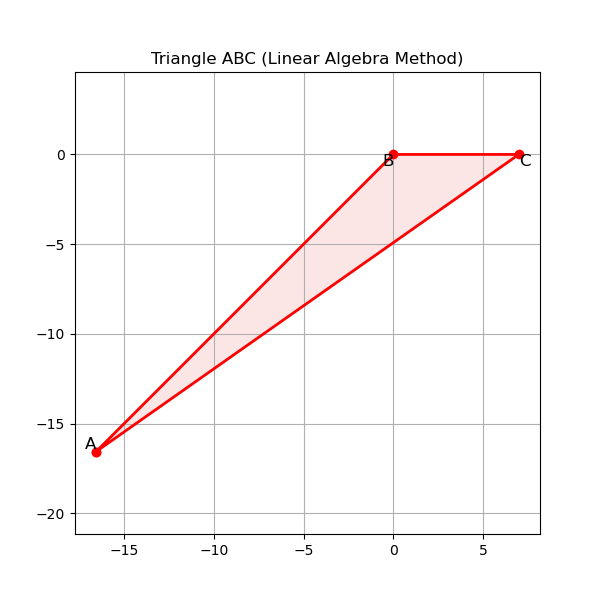
\includegraphics[width=0.58\linewidth]{./figs/Figure_1.png}
        \caption{}
        \label{fig:fig1}
    \end{figure}
\end{frame}


\end{document}
